%%%%%%%%%%%%%%%%%%%%%%%%%%%%%%%%%%%%%%%%%%%%%%%%%%%%%%%%%%%%%%%%%%%%%%%%
\chapter{Goclassy}
%%%%%%%%%%%%%%%%%%%%%%%%%%%%%%%%%%%%%%%%%%%%%%%%%%%%%%%%%%%%%%%%%%%%%%%%

\begin{center}
    \begin{minipage}{0.5\textwidth}
        \begin{small}
            In which we introduce Goclassy the first of the OSCAR pipelines, as well as OSCAR 2019 which was the first relase of the OSCAR corpus based on the OSCAR dump of November 2018.
        \end{small}
    \end{minipage}
    \vspace{0.5cm}
\end{center}

%\noindent Common Crawl is a considerably large, heterogeneous multilingual corpus comprised of crawled documents from the internet, surpassing 20TB of data and distributed as a set of more than 50 thousand plain text files where each contains many documents written in a wide variety of languages. Even though each document has a metadata block associated to it, this data lacks any information about the language in which each document is written, making it extremely difficult to use Common Crawl for monolingual applications. We propose a general, highly parallel, multithreaded pipeline to clean and classify Common Crawl by language; we specifically design it so that it runs efficiently on medium to low resource infrastructures where I/O speeds are the main constraint. We develop the pipeline so that it can be easily reapplied to any kind of  heterogeneous corpus and so that it can be parameterised to a wide range of infrastructures. We also distribute a 6.3TB version of Common Crawl, filtered, classified by language, shuffled at line level in order to avoid copyright issues, and ready to be used for NLP applications.

\section{Asynchronous pipeline}

\begin{figure*}
    \centering
    \begin{tikzpicture}[auto,scale=0.85, every node/.style={transform shape},font=\sffamily]
        \tikzstyle{nod}=[minimum width=1.65cm,minimum height=6cm,rectangle,rounded corners=10pt,
        fill=red!20, align=center, text width=1.65cm,text centered]
        \tikzstyle{ft} = [minimum width=1.5cm,minimum height=1cm,rectangle,rounded corners=10pt,
        fill=blue!20, align=center, text width=1.5cm,text centered]
        \tikzstyle{fin}=[minimum width=4cm,minimum height=4cm,rectangle,rounded corners=10pt,
        fill=green!20, align=center, text width=4cm,text centered]
        \tikzstyle{arr}=[->,>=stealth,thick]
        \tikzstyle{arr1}=[->,>=stealth,thick, dashed]

        \node[nod] (CC) at (0,0) {Common Crawl};

        \node[minimum width=2cm, text width=2cm,text centered] (TEX1) at (2.5,3.45) {\small Compressed Files};
        \node (GZ1) at (2.5,2.3) {\Huge \faFileArchive[regular]};
        \node (GZ2) at (2.5,1) {\Huge \faFileArchive[regular]};
        \node (GZ3) at (2.5, -0.3) {\Huge \faFileArchive[regular]};
        \node (DGZ) at (2.5, -1.2) {\Huge $\vdots$};
        \node (GZ4) at (2.5,-2.3) {\Huge \faFileArchive[regular]};


        \node[minimum width=1cm, text width=1cm,text centered] (TEX1) at (4.5,3.45) {\small WET Files};
        \node (T1) at (4.5,2.3) {\Huge \faFile*};
        \node (T2) at (4.5,1) {\Huge \faFile*};
        \node (T3) at (4.5, -0.3) {\Huge \faFile*};
        \node (DT) at (4.5, -1.2) {\Huge $\vdots$};
        \node (T4) at (4.5,-2.3) {\Huge \faFile*};

        \node[ft] (F1) at (7,2.3) {fastText};
        \node[ft] (F2) at (7,1) {fastText};
        \node[ft] (F3) at (7,-0.3) {fastText};
        \node (DF) at (7, -1.2) {\Huge $\vdots$};
        \node[ft] (F4) at (7,-2.3) {fastText};

        \node[minimum width=2.3cm, text width=2.3cm,text centered] (TEX1) at (10.25,3.45) {\small Filtered Files Language Tags};
        \node (TA1) at (10.25,2.3) {\Huge \faFile*[regular] $\,$ \faTags};
        \node (TA2) at (10.25,1) {\Huge \faFile*[regular] $\,$ \faTags};
        \node (TA3) at (10.25, -0.3) {\Huge \faFile*[regular] $\,$ \faTags};
        \node (DTA) at (10.25, -1.2) {\Huge $\vdots$};
        \node (TA4) at (10.25,-2.3) {\Huge \faFile*[regular] $\,$ \faTags};


        \node[minimum width=2.3cm, text width=2.3cm,text centered] (TEX1) at (15,3.45) {\small Files Classified by Language};
        \node[fin] (FF) at (15,0) {};
        \node (TF) at (15,1.3) {\Huge \faLanguage $\,\cdots$\faLanguage};
        \node (TF3) at (15, 0) {\Huge \faLanguage $\,\cdots$\faLanguage};
        \node (TF3) at (15, -1.3) {\Huge \faLanguage $\,\cdots$\faLanguage};


        \draw[arr] (1,2.3)--(GZ1);
        \draw[arr] (1,1)--(GZ2);
        \draw[arr] (1,-0.3)--(GZ3);
        \draw[arr] (1,-2.3)--(GZ4);


        \draw[arr] (GZ1)--(T1);
        \draw[arr] (GZ2)--(T2);
        \draw[arr] (GZ3)--(T3);
        \draw[arr] (GZ4)--(T4);


        \draw[arr1] (5,2.5)--(6.1,2.5);
        \draw[arr1] (5,2.3)--(6.1,2.3);
        \draw[arr1] (5,2.1)--(6.1,2.1);

        \draw[arr1] (5,1.2)--(6.1,1.2);
        \draw[arr1] (5,1)--(6.1,1);
        \draw[arr1] (5,0.8)--(6.1,0.8);

        \draw[arr1] (5,-0.1)--(6.1,-0.1);
        \draw[arr1] (5,-0.3)--(6.1,-0.3);
        \draw[arr1] (5,-0.5)--(6.1,-0.5);

        \draw[arr1] (5,-2.1)--(6.1,-2.1);
        \draw[arr1] (5,-2.3)--(6.1,-2.3);
        \draw[arr1] (5,-2.5)--(6.1,-2.5);


        \draw[arr] (8,2.5)--(9.1,2.5);
        \draw[arr] (8,2.3)--(9.1,2.3);
        \draw[arr] (8,2.1)--(9.1,2.1);

        \draw[arr] (8,1.2)--(9.1,1.2);
        \draw[arr] (8,1)--(9.1,1);
        \draw[arr] (8,0.8)--(9.1,0.8);

        \draw[arr] (8,-0.1)--(9.1,-0.1);
        \draw[arr] (8,-0.3)--(9.1,-0.3);
        \draw[arr] (8,-0.5)--(9.1,-0.5);

        \draw[arr] (8,-2.1)--(9.1,-2.1);
        \draw[arr] (8,-2.3)--(9.1,-2.3);
        \draw[arr] (8,-2.5)--(9.1,-2.5);


        \draw[arr] (TA1.0)--(FF);
        \draw[arr] (TA2.0)--(FF);
        \draw[arr] (TA3.0)--(FF);
        \draw[arr] (TA4.0)--(FF);
    \end{tikzpicture}
    \caption{A scheme of the \emph{goclassy} pipeline. The red square represents the Compressed WET files stored on Amazon Web Services. The {\faFileArchive[regular]} icons represent the gzip files stored locally, the {\faFile*} represent one of the 50K WET files. The {\faFile*[regular]} represents the filtered file and the {\faTags} represents a file of language tags, one tag per line in \faFile*[regular]. The {\faLanguage} represents one of the 166 classified files. Each arrow represents an asynchronous non blocking worker and dotted arrows represent a line filtering process.}
    \label{fig:D1}
\end{figure*}

We propose a new pipeline derived from the fastText one which we call \texttt{goclassy}, we reuse the fastText linear classifier \citep{joulin-etal-2016-fasttext, joulin-etal-2017-bag} and the pre-trained fastText model for language recognition \citep{grave-etal-2018-learning}, but we completely rewrite and parallelise their pipeline in an asynchronous manner.

The order of operations is more or less the same as in the fastText pre-processing pipeline but instead of clustering multiple operations into a single blocking process, we launch a worker for each operation and we bound the number of possible parallel operations at a given time by the number of available threads instead of the number of CPUs. We implement goclassy using the Go programming language\footnote{\url{https://golang.org/}} so we let the Go runtime\footnote{\url{https://golang.org/src/runtime/mprof.go}} handle the scheduling of the processes. Thus in our pipeline we don't have to wait for a whole WET file to download, decompress and classify in order to start downloading and processing the next one, a new file will start downloading and processing as soon as the scheduler is able to allocate a new process.

When using electromechanical mediums of storage, I/O blocking is one of the main problems one encounters. To overcome this, we introduced buffers in all our I/O operations, a feature that is not present in the fastText pre-processing pipeline. We also create, from the start, a file for each of the 176 languages that the pre-trained fastText language classifier is capable of recognising, and we always leave them open, as we find that getting a file descriptor to each time we want to write, if we wanted leave them open just when needed, introduces a big overhead.

We also do the filtering and cleaning processes at line level before feeding each line to the classifier, which makes us create a new filtered file so that we can have a correspondence with the tag file, which in turn will consume more space, but that will also reduce the amount of unnecessary classifications performed by fastText. The filtered and file tags are then read and lines are appended to its corresponding language file. The writing in the classification step is asynchronous, meaning that process writing a line to the filtered files does not wait for the classifier to write a tag on the tag file. Figure \ref{fig:D1} shows the pipeline up to this point.

After all WET files are processed, we then use Isaac Whitfield's deduplication tool runiq\footnote{\url{https://github.com/whitfin/runiq}} which is based on Yann Collet's xxhash64\footnote{\url{https://github.com/Cyan4973/xxHash}}, an extremely fast non-cryptographic hash algorithm that is resistant to collisions. We finally use the Mark Adler's pigz\footnote{\url{https://zlib.net/pigz/}} for data compression, as opposed to the canonical UNIX tools proposed in the original fastText pipeline. We add both tools to our concurrent pipeline, executing multiple instances of them in parallel, in order to ensure we use the most of our available resources at a given time.

Beyond improving the computational time required to classify this corpus, we propose a simple improvement on the cleaning scheme in the fastText pre-processing pipeline. This improvement allows our pipeline to better take into account the multilingual nature of Common Crawl; that is, we count UTF-8 characters instead of bytes for setting the lower admissible bound for the length of a line to be fed into the classifier. This straightforward modification on the fastText pre-processing pipeline assures we take into account the multiple languages present in Common Crawl that use non-ASCII encoded characters.

Given that our implementation is written in Go, we release binary distributions \footnote{\url{https://github.com/pjox/goclassy}} of goclassy for all major operating systems. Both pigz and runiq are also available for all major operating systems.

\section{Benchmarks}

\begin{table*}[ht!]
    \centering\small
    \begin{tabular}{lrrrcrrrcrrr}\toprule
                 & \multicolumn{3}{c}{10 files} & \phantom{a}             & \multicolumn{3}{c}{100 files} & \phantom{a} & \multicolumn{3}{c}{200 files}                                                                                                                                        \\
        \cmidrule{2-4} \cmidrule{6-8} \cmidrule{10-12}
                 & \multicolumn{1}{c}{Min}      & \multicolumn{1}{c}{Max} & \multicolumn{1}{c}{Mean}      &             & \multicolumn{1}{c}{Min}       & \multicolumn{1}{c}{Max} & \multicolumn{1}{c}{Mean} &  & \multicolumn{1}{c}{Min} & \multicolumn{1}{c}{Max} & \multicolumn{1}{c}{Mean} \\ \midrule
        \emph{real}                                                                                                                                                                                                                                                                            \\
        fastText & 2m50s                        & 6m45s                   & 3m31s                         &             & 13m46s                        & 38m38s                  & 17m39s                   &  & 26m20s                  & 47m48s                  & 31m4s                    \\
        goclassy & 1m23s                        & 3m12s                   & 1m42s                         &             & 7m42s                         & 12m43s                  & 9m8s                     &  & 15m3s                   & 15m47s                  & 15m16s                   \\
        \emph{user}                                                                                                                                                                                                                                                                            \\
        fastText & 26m45s                       & 27m2s                   & 26m53s                        &             & 4h21m                         & 4h24m                   & 4h23m                    &  & 8h42m                   & 8h48m                   & 8h45m                    \\
        goclassy & 10m26s                       & 12m53s                  & 11m0s                         &             & 1h46m                         & 1h54m                   & 1h49m                    &  & 3h37m                   & 3h40m                   & 3h38m                    \\
        \emph{sys}                                                                                                                                                                                                                                                                             \\
        fastText & 40.14s                       & 40.85s                  & 40.56s                        &             & 6m14s                         & 6m17s                   & 6m15s                    &  & 12m26s                  & 12m45s                  & 12m31s                   \\
        goclassy & 37.34s                       & 45.98s                  & 39.67s                        &             & 5m7s                          & 5m34s                   & 5m16s                    &  & 9m57s                   & 10m14s                  & 10m5s                    \\
        \bottomrule
    \end{tabular}
    \caption{Benchmarks are done using the UNIX \texttt{time} tool, are repeated 10 times each and are done for random samples of 10, 100 and 200 WET files. Only the classifying and filtering part are benchmarked. The table shows the minimum, maximum and mean time for the user, real and sys time over the 10 runs. Here ``fastText'' is used as short for the pipeline.}
    \label{tab:Bench}
\end{table*}

We test both pipelines against one another in an infrastructure using traditional electromechanical storage mediums that are connected to the main processing machine via an Ethernet interface, that is, a low I/O speed environment as compared to an infrastructure where one would have an array of SSDs connected directly to the main processing machine via a high speed interface. We use a machine with an Intel\textsuperscript{\textregistered} Xeon\textsuperscript{\textregistered} Processor E5-2650 2.00 GHz, 20M Cache, and 203.1 GiB of RAM. We make sure that no other processes apart from the benchmark and the Linux system processes are run. We do not include downloading, decompression or deduplication in our benchmarks as downloading takes far too much time, and deduplication and compression were performed with third party tools that don't make part of our main contribution. We are mainly interested in seeing how the way the data is fed to the classifier impacts the overall processing time.

Benchmarks in table \ref{tab:Bench} of our goclassy pipeline show a drastic reduction in processing time compared to the original fastText prepossessing pipeline. We show that in our particular infrastructure, we are capable of reducing the \emph{real} time as measured by the \texttt{time} UNIX tool almost always by half. The \emph{user} time which represents the amount of CPU time spent in user-mode code (outside the kernel) within the process is almost three times lower for our goclassy pipeline, this particular benchmark strongly suggest a substantial reduction in energy consumption of goclassy with respect to the fastText pipeline.

As we understand that even an infrastructure with more than 20TB of free space in traditional electromechanical storage is not available to everyone and we propose a simple parametrization in our pipeline that actively deletes already processed data and that only downloads and decompresses files when needed, thus ensuring that no more than 10TB of storage are used at a given time. We nevertheless note that delaying decompression increases the amount of computation time, which is a trade-off that some users might make as it might be more suitable for their available infrastructure.

\section{OSCAR}

\begin{table*}[t!]
    \centering\tiny
    \resizebox{\linewidth}{!}{
        \begin{tabular}{@{}lrrrrclrrrr@{}}\toprule
            \multirow{2}{*}{Language} & \multicolumn{2}{c}{Size} & \multicolumn{2}{c}{Words} & \phantom{a}              & \multirow{2}{*}{Language} & \multicolumn{2}{c}{Size} & \multicolumn{2}{c}{Words}                                                                                                               \\
            \cmidrule(l{2pt}r{2pt}){2-3} \cmidrule(l{2pt}r{2pt}){4-5} \cmidrule(l{2pt}r{2pt}){8-9} \cmidrule(l{2pt}r{2pt}){10-11}
                                      & \multicolumn{1}{c}{Orig} & \multicolumn{1}{c}{Dedup} & \multicolumn{1}{c}{Orig} & \multicolumn{1}{c}{Dedup} & \phantom{a}              &                           & \multicolumn{1}{c}{Orig} & \multicolumn{1}{c}{Dedup} & \multicolumn{1}{c}{Orig} & \multicolumn{1}{c}{Dedup} \\\midrule
            Afrikaans                 & 241M                     & 163M                      & 43,482,801               & 29,533,437                &                          & Lower Sorbian             & 13K                      & 7.1K                      & 1,787                    & 966                       \\
            Albanian                  & 2.3G                     & 1.2G                      & 374,196,110              & 186,856,699               &                          & Luxembourgish             & 29M                      & 21M                       & 4,403,577                & 3,087,650                 \\
            Amharic                   & 360M                     & 206M                      & 28,301,601               & 16,086,628                &                          & Macedonian                & 2.1G                     & 1.2G                      & 189,289,873              & 102,849,595               \\
            Arabic                    & 82G                      & 32G                       & 8,117,162,828            & 3,171,221,354             &                          & Maithili                  & 317K                     & 11K                       & 69,161                   & 874                       \\
            Aragonese                 & 1.3M                     & 801K                      & 52,896                   & 45,669                    &                          & Malagasy                  & 21M                      & 13M                       & 3,068,360                & 1,872,044                 \\
            Armenian                  & 3.7G                     & 1.5G                      & 273,919,388              & 110,196,043               &                          & Malay                     & 111M                     & 42M                       & 16,696,882               & 6,045,753                 \\
            Assamese                  & 113M                     & 71M                       & 6,956,663                & 4,366,570                 &                          & Malayalam                 & 4.9G                     & 2.5G                      & 189,534,472              & 95,892,551                \\
            Asturian                  & 2.4M                     & 2.0M                      & 381,005                  & 325,237                   &                          & Maltese                   & 24M                      & 17M                       & 2,995,654                & 2,163,358                 \\
            Avaric                    & 409K                     & 324K                      & 24,720                   & 19,478                    &                          & Marathi                   & 2.7G                     & 1.4G                      & 162,609,404              & 82,130,803                \\
            Azerbaijani               & 2.8G                     & 1.5G                      & 322,641,710              & 167,742,296               &                          & Mazanderani               & 691K                     & 602K                      & 73,870                   & 64,481                    \\
            Bashkir                   & 128M                     & 90M                       & 9,796,764                & 6,922,589                 &                          & Minangkabau               & 608K                     & 310K                      & 5,682                    & 4,825                     \\
            Basque                    & 848M                     & 342M                      & 120,456,652              & 45,359,710                &                          & Mingrelian                & 5.8M                     & 4.4M                      & 299,098                  & 228,629                   \\
            Bavarian                  & 503                      & 503                       & 399                      & 399                       &                          & Mirandese                 & 1.2K                     & 1.1K                      & 171                      & 152                       \\
            Belarusian                & 1.8G                     & 1.1G                      & 144,579,630              & 83,499,037                &                          & Modern Greek              & 62G                      & 27G                       & 5,479,180,137            & 2,412,419,435             \\
            Bengali                   & 11G                      & 5.8G                      & 623,575,733              & 363,766,143               &                          & Mongolian                 & 2.2G                     & 838M                      & 181,307,167              & 68,362,013                \\
            Bihari                    & 110K                     & 34K                       & 8,848                    & 2,875                     &                          & Nahuatl languages         & 12K                      & 11K                       & 1,234                    & 1,193                     \\
            Bishnupriya               & 4.1M                     & 1.7M                      & 198,286                  & 96,940                    &                          & Neapolitan                & 17K                      & 13K                       & 5,282                    & 4,147                     \\
            Bosnian                   & 447K                     & 116K                      & 106,448                  & 20,485                    &                          & Nepali                    & 1.8G                     & 1.2G                      & 107,448,208              & 71,628,317                \\
            Breton                    & 29M                      & 16M                       & 5,013,241                & 2,890,384                 &                          & Newari                    & 5.5M                     & 4.1M                      & 564,697                  & 288,995                   \\
            Bulgarian                 & 32G                      & 14G                       & 2,947,648,106            & 1,268,114,977             &                          & Northern Frisian          & 4.4K                     & 4.4K                      & 1,516                    & 1,516                     \\
            Burmese                   & 1.9G                     & 1.1G                      & 56,111,184               & 30,102,173                &                          & Northern Luri             & 76K                      & 63K                       & 8,022                    & 6,740                     \\
            Catalan                   & 8.0G                     & 4.3G                      & 1,360,212,450            & 729,333,440               &                          & Norwegian                 & 8.0G                     & 4.7G                      & 1,344,326,388            & 804,894,377               \\
            Cebuano                   & 39M                      & 24M                       & 6,603,567                & 3,675,024                 &                          & Norwegian Nynorsk         & 85M                      & 54M                       & 14,764,980               & 9,435,139                 \\
            Central Bikol             & 885                      & 885                       & 312                      & 312                       &                          & Occitan                   & 5.8M                     & 3.7M                      & 750,301                  & 512,678                   \\
            Central Khmer             & 1.1G                     & 581M                      & 20,690,610               & 10,082,245                &                          & Oriya                     & 248M                     & 188M                      & 14,938,567               & 11,321,740                \\
            Central Kurdish           & 487M                     & 226M                      & 48,478,334               & 18,726,721                &                          & Ossetian                  & 13M                      & 11M                       & 1,031,268                & 878,765                   \\
            Chavacano                 & 520                      & 520                       & 130                      & 130                       &                          & Pampanga                  & 760                      & 304                       & 130                      & 52                        \\
            Chechen                   & 8.3M                     & 6.7M                      & 711,051                  & 568,146                   &                          & Panjabi                   & 763M                     & 460M                      & 61,847,806               & 37,555,835                \\
            Chinese                   & 508G                     & 249G                      & 14,986,424,850           & 6,350,215,113             &                          & Persian                   & 79G                      & 38G                       & 9,096,554,121            & 4,363,505,319             \\
            Chuvash                   & 39M                      & 26M                       & 3,041,614                & 2,054,810                 &                          & Piemontese                & 2.1M                     & 1.9M                      & 362,013                  & 337,246                   \\
            Cornish                   & 44K                      & 14K                       & 8,329                    & 2,704                     &                          & Polish                    & 109G                     & 47G                       & 15,277,255,137           & 6,708,709,674             \\
            Croatian                  & 226M                     & 110M                      & 34,232,765               & 16,727,640                &                          & Portuguese                & 124G                     & 64G                       & 20,641,903,898           & 10,751,156,918            \\
            Czech                     & 53G                      & 24G                       & 7,715,977,441            & 3,540,997,509             &                          & Pushto                    & 361M                     & 242M                      & 46,559,441               & 31,347,348                \\
            Danish                    & 16G                      & 9.5G                      & 2,637,463,889            & 1,620,091,317             &                          & Quechua                   & 78K                      & 67K                       & 10,186                   & 8,691                     \\
            Dhivehi                   & 126M                     & 79M                       & 7,559,472                & 4,726,660                 &                          & Romanian                  & 25G                      & 11G                       & 3,984,317,058            & 1,741,794,069             \\
            Dimli                     & 146                      & 146                       & 19                       & 19                        &                          & Romansh                   & 7.4K                     & 6.5K                      & 1,093                    & 960                       \\
            Dutch                     & 78G                      & 39G                       & 13,020,136,373           & 6,598,786,137             &                          & Russia Buriat             & 13K                      & 11K                       & 963                      & 809                       \\
            Eastern Mari              & 7.2M                     & 6.0M                      & 565,992                  & 469,297                   &                          & Russian                   & 1.2T                     & 568G                      & 92,522,407,837           & 46,692,691,520            \\
            Egyptian Arabic           & 66M                      & 33M                       & 7,305,151                & 3,659,419                 &                          & Sanskrit                  & 93M                      & 37M                       & 4,331,569                & 1,713,930                 \\
            Emilian-Romagnol          & 25K                      & 24K                       & 6,376                    & 6,121                     &                          & Scottish Gaelic           & 1.9M                     & 1.3M                      & 310,689                  & 207,110                   \\
            English                   & 2.3T                     & 1.2T                      & 418,187,793,408          & 215,841,256,971           &                          & Serbian                   & 3.9G                     & 2.2G                      & 364,395,411              & 207,561,168               \\
            Erzya                     & 1.4K                     & 1.2K                      & 90                       & 78                        &                          & Serbo-Croatian            & 25M                      & 5.8M                      & 5,292,184                & 1,040,573                 \\
            Esperanto                 & 299M                     & 228M                      & 48,486,161               & 37,324,446                &                          & Sicilian                  & 3.3K                     & 2.8K                      & 554                      & 468                       \\
            Estonian                  & 4.8G                     & 2.3G                      & 643,163,730              & 309,931,463               &                          & Sindhi                    & 347M                     & 263M                      & 43,530,158               & 33,028,015                \\
            Finnish                   & 27G                      & 13G                       & 3,196,666,419            & 1,597,855,468             &                          & Sinhala                   & 1.4G                     & 802M                      & 93,053,465               & 50,864,857                \\
            French                    & 282G                     & 138G                      & 46,896,036,417           & 23,206,776,649            &                          & Slovak                    & 9.1G                     & 4.5G                      & 1,322,247,763            & 656,346,179               \\
            Galician                  & 620M                     & 384M                      & 102,011,291              & 63,600,602                &                          & Slovenian                 & 2.5G                     & 1.3G                      & 387,399,700              & 193,926,684               \\
            Georgian                  & 3.6G                     & 1.9G                      & 171,950,621              & 91,569,739                &                          & Somali                    & 61K                      & 16K                       & 1,202                    & 472                       \\
            German                    & 308G                     & 145G                      & 44,878,908,446           & 21,529,164,172            &                          & South Azerbaijani         & 27M                      & 19M                       & 2,175,054                & 1,528,709                 \\
            Goan Konkani              & 2.2M                     & 1.8M                      & 124,277                  & 102,306                   &                          & Spanish                   & 278G                     & 149G                      & 47,545,122,279           & 25,928,290,729            \\
            Guarani                   & 36K                      & 24K                       & 7,382                    & 4,680                     &                          & Sundanese                 & 211K                     & 141K                      & 30,321                   & 20,278                    \\
            Gujarati                  & 1.1G                     & 722M                      & 72,045,701               & 50,023,432                &                          & Swahili                   & 13M                      & 8.1M                      & 2,211,927                & 1,376,963                 \\
            Haitian                   & 3.9K                     & 3.3K                      & 1,014                    & 832                       &                          & Swedish                   & 44G                      & 25G                       & 7,155,994,312            & 4,106,120,608             \\
            Hebrew                    & 20G                      & 9.8G                      & 2,067,753,528            & 1,032,018,056             &                          & Tagalog                   & 573M                     & 407M                      & 98,949,299               & 70,121,601                \\
            Hindi                     & 17G                      & 8.9G                      & 1,372,234,782            & 745,774,934               &                          & Tajik                     & 379M                     & 249M                      & 31,758,142               & 21,029,893                \\
            Hungarian                 & 40G                      & 18G                       & 5,163,936,345            & 2,339,127,555             &                          & Tamil                     & 9.3G                     & 5.1G                      & 420,537,132              & 226,013,330               \\
            Icelandic                 & 1.5G                     & 846M                      & 219,900,094              & 129,818,331               &                          & Tatar                     & 670M                     & 305M                      & 51,034,893               & 23,825,695                \\
            Ido                       & 147K                     & 130K                      & 25,702                   & 22,773                    &                          & Telugu                    & 2.5G                     & 1.6G                      & 123,711,517              & 79,094,167                \\
            Iloko                     & 874K                     & 636K                      & 142,942                  & 105,564                   &                          & Thai                      & 36G                      & 16G                       & 951,743,087              & 368,965,202               \\
            Indonesian                & 30G                      & 16G                       & 4,574,692,265            & 2,394,957,629             &                          & Tibetan                   & 187M                     & 138M                      & 1,483,589                & 936,556                   \\
            Interlingua               & 662K                     & 360K                      & 180,231                  & 100,019                   &                          & Tosk Albanian             & 5.0M                     & 2.8M                      & 841,750                  & 459,001                   \\
            Interlingue               & 24K                      & 1.6K                      & 5,352                    & 602                       &                          & Turkish                   & 60G                      & 27G                       & 7,577,388,700            & 3,365,734,289             \\
            Irish                     & 88M                      & 60M                       & 14,483,593               & 10,017,303                &                          & Turkmen                   & 11M                      & 6.8M                      & 1,113,869                & 752,326                   \\
            Italian                   & 137G                     & 69G                       & 22,248,707,341           & 11,250,012,896            &                          & Tuvinian                  & 12K                      & 7.9K                      & 759                      & 540                       \\
            Japanese                  & 216G                     & 106G                      & 4,962,979,182            & 1,123,067,063             &                          & Uighur                    & 122M                     & 83M                       & 8,657,141                & 5,852,225                 \\
            Javanese                  & 659K                     & 583K                      & 104,896                  & 86,654                    &                          & Ukrainian                 & 53G                      & 28G                       & 4,204,381,276            & 2,252,380,351             \\
            Kalmyk                    & 113K                     & 112K                      & 10,277                   & 10,155                    &                          & Upper Sorbian             & 4.2M                     & 1.8M                      & 545,351                  & 236,867                   \\
            Kannada                   & 1.7G                     & 1.1G                      & 81,186,863               & 49,343,462                &                          & Urdu                      & 2.7G                     & 1.7G                      & 331,817,982              & 218,030,228               \\
            Karachay-Balkar           & 2.6M                     & 2.3M                      & 185,436                  & 166,496                   &                          & Uzbek                     & 21M                      & 12M                       & 2,450,256                & 1,381,644                 \\
            Kazakh                    & 2.7G                     & 1.5G                      & 191,126,469              & 108,388,743               &                          & Venetian                  & 18K                      & 17K                       & 3,492                    & 3,199                     \\
            Kirghiz                   & 600M                     & 388M                      & 44,194,823               & 28,982,620                &                          & Vietnamese                & 68G                      & 32G                       & 12,036,845,359           & 5,577,159,843             \\
            Komi                      & 2.3M                     & 1.2M                      & 201,404                  & 95,243                    &                          & Volapük                   & 2.0M                     & 2.0M                      & 321,121                  & 318,568                   \\
            Korean                    & 24G                      & 12G                       & 2,368,765,142            & 1,120,375,149             &                          & Walloon                   & 273K                     & 203K                      & 50,720                   & 37,543                    \\
            Kurdish                   & 94M                      & 60M                       & 15,561,003               & 9,946,440                 &                          & Waray                     & 2.5M                     & 2.2M                      & 397,315                  & 336,311                   \\
            Lao                       & 174M                     & 114M                      & 4,133,311                & 2,583,342                 &                          & Welsh                     & 213M                     & 133M                      & 37,422,441               & 23,574,673                \\
            Latin                     & 26M                      & 8.3M                      & 4,122,201                & 1,328,038                 &                          & Western Frisian           & 35M                      & 26M                       & 5,691,077                & 4,223,816                 \\
            Latvian                   & 4.0G                     & 1.8G                      & 520,761,977              & 236,428,905               &                          & Western Mari              & 1.2M                     & 1.1M                      & 93,338                   & 87,780                    \\
            Lezghian                  & 3.3M                     & 3.0M                      & 247,646                  & 224,871                   &                          & Western Panjabi           & 12M                      & 9.0M                      & 1,426,986                & 1,111,112                 \\
            Limburgan                 & 29K                      & 27K                       & 4,730                    & 4,283                     &                          & Wu Chinese                & 109K                     & 32K                       & 11,189                   & 4,333                     \\
            Lithuanian                & 8.8G                     & 3.9G                      & 1,159,661,742            & 516,183,525               &                          & Yakut                     & 42M                      & 26M                       & 2,547,623                & 1,789,174                 \\
            Lojban                    & 736K                     & 678K                      & 154,330                  & 141,973                   &                          & Yiddish                   & 141M                     & 84M                       & 13,834,320               & 8,212,970                 \\
            Lombard                   & 443K                     & 433K                      & 75,229                   & 73,665                    &                          & Yoruba                    & 55K                      & 27K                       & 8,906                    & 3,518                     \\
            Low German                & 18M                      & 13M                       & 2,906,347                & 2,146,417                 &                          & Yue Chinese               & 3.7K                     & 2.2K                      & 186                      & 128                       \\
            \midrule
            \textbf{Total}            & 6.3T                     & 3.2T                      & 844,315,434,723          & 425,651,344,234           &                          &                           &                          &                           &                          &                           \\
            \bottomrule
        \end{tabular}
    }
    \caption{Size of the OSCAR corpus by language measured in bytes and number of words. Standard UNIX human-readable notation is used for the size in byte. We define ``words'' as spaced separated tokens, which gives a good estimate of the size of each corpus for languages using Latin or Cyrillic alphabets, but might give a misleading size for other languages such as Chinese or Japanese.}
    \label{tab:langs-goclassy}
\end{table*}

Finally, we are aware that some users might not even have access to a big enough infrastructure to run our pipelines or just to store all the Common Crawl data. Moreover, even if previously used and cited in NLP and Machine Learning research, we note that there is currently no public distribution of Common Crawl that is filtered, classified by language and ready to use for Machine Learning or NLP applications. Thus we decide to publish a pre-processed version of the November 2018 copy of Common Crawl which is comprised of usable data in 166 different languages, we publish\footnote{\url{https://team.inria.fr/almanach/oscar/}} our version under the name OSCAR which is short for \emph{Open Super-large Crawled ALMAnaCH\footnote{\url{https://team.inria.fr/almanach/}} coRpus}.

After processing all the data with goclassy, the size of the whole Common Crawl corpus is reduced to 6.3TB, but in spite of this considerable reduction, OSCAR still dwarfs all previous mentioned corpora having more 800 billion ``words'' or spaced separated tokens and noting that this in fact is an understatement of how big OSCAR is, as some of the largest languages within OSCAR such as Chinese and Japanese do not use spaces. The sizes in bytes for both the original and the deduplicated versions of OSCAR can be found in table \ref{tab:langs-goclassy}. OSCAR is published under the \emph{Creative Commons CC0 license (``no rights reserved'')}\footnote{\url{http://creativecommons.org/publicdomain/zero/1.0/}}, so it is free to use for all applications.

\section{Conclusions}

We are sure that our work will greatly benefit researchers working on an either constrain infrastructure or a low budget setting. We are also confident, that by publishing a classified version of Common Crawl, we will substantially increase the amount of available public data for medium to low resource languages, thus improving and facilitating NLP research for them. Furthermore, as our pipeline speeds-up and simplifies the treatment of Common Crawl, we believe that our contribution can be further parallelised and adapted to treat multiple snapshots of Common Crawl opening the door to what would be otherwise costly diachronic studies of the use of a given language throughout the internet.

Finally, we note that both our proposed pipeline is data independent, which means that they can be reused to process, clean and classify any sort of big multilingual corpus that is available in plain text form and that is UTF-8 encoded; meaning that the impact of our work goes way beyond a single corpus.